\documentclass[12pt]{article}
\usepackage{../preamble}
\graphicspath{{pics/hw1/}}
\begin{document}
% \maketitle
\chead{Problem Set 1}

%%%%%%%%%%%%%%%%%%%%%%%%%%%%%%%%%%%%%%%%%%%%%%%
%                  Definitions                %
%%%%%%%%%%%%%%%%%%%%%%%%%%%%%%%%%%%%%%%%%%%%%%%
%\includegraphics[width=\mywidth\textwidth]{}

% \begin{figure}[h!]
% \centering
% \input{pics/PS2/p7b}
% \caption{}
% \label{fig-}
% \end{figure}

% \begin{enumerate}[label=\alph*.]
%     \setcounter{enumi}{1}
%     \item 
% \end{enumerate}

%%%%%%%%%%%%%%%%%
%     Part a    %
%%%%%%%%%%%%%%%%%


%%%%%%%%%%%%%%%%%%%%%%%%%%%%%%%%%%%%%%%%%%%%%%%
%                Problem 1                    %
%%%%%%%%%%%%%%%%%%%%%%%%%%%%%%%%%%%%%%%%%%%%%%%
\section*{Problem 1}
\problem{Clean subsidies versus dirty taxes}{
    Many environmental policies take the form of subsidies for clean goods or activities, rather than taxes on the dirty good or activity. Presumably such instruments are popular in part because it is more politically appealing to give away a subsidy than to collect a tax. The aim of this exercise is to get you to consider the economic efficiency of using “green subsidies” in lieu of “brown taxes” (or “clean subsidies” in lieu of “dirty taxes”).\\

Consider the following model (which we used in lecture). There P are heterogeneous producers indexed $j = 1, ..., J$, which produce homogeneous good $x_j ; X \equiv\sum_{j=1}^J x_j$ , according to production cost $c_j(x_j )$ (with $c_j' > 0, c_j'' > 0$). A representative consumer has utility $U(X)$ (with $U' > 0$, $U'' \leq 0$). Production creates an externality according to $e_j(x_j)$, (with $e_j' > 0$, $e_j'' \leq 0$). Firms can abate emission $a_ j$, at cost $g_j(a_j)$ (with $g_j' > 0$, $g_j'' > 0$). Net emissions from firm $j$ are thus $e_j(x_j) - a_j$, and total damages to the consumer are $\phi\sum_{j=1}^J (e_j(x_j) - a_j)$.\\

Suppose that the only instrument the planner has available is a subsidy, denoted $s$, which can be awarded to each firm based on its level of abatement $a_j$ , for a total subsidy of $sa_j$ . The planner can choose the level of the subsidy, but no other policies are available.\\

\textbf{Evaluate the following two claims; that is, prove their veracity or falsity using the model:}
\begin{enumerate}
    \item An abatement subsidy can be used to decentralize the optimal allocation.
    \item An abatement subsidy can be used to generate the socially optimal level of abatement at each firm.
\end{enumerate}
}


\def\sumj{\sum\limits_j} \def\sumi{\sum\limits_i} \def\sumk{\sum\limits_k}
\def\cj{c_j(x_j)} \def\cjprime{c_j'(x_j)}
\def\gj{g_j(a_j)} \def\gjprime{g_j'(a_j)}
\def\ej{e_j(x_j)} \def\ejprime{e_j'(x_j)}
\def\dda{\frac{\partial}{\partial a_j}} \def\ddx{\frac{\partial}{\partial x_j}}
\begin{align*} 
\intertext{Let $A\equiv\sum_j a_j$ and $E\equiv\sum_j e_j(x_j)$. To find the optimal allocation, consider the social planner's problem:}
    \max_{a_j,x_j} SWF &= \text{Benefit of consuming $X$} - \text{Cost of producing $X$}
        - \text{Cost of abating $A$} - \text{Cost of externality E}\\
    &= U(X) - \sumj(\cj +\gj) - \phi\sumj(\ej - a_j)
\intertext{The First Order Conditions describing the optimal allocation and firm-level abatement are then}
    \dda SWF &= \phi - \gjprime = 0 \implies \gjprime = \phi\\
    \ddx SWF &= \ddx U - \cjprime - \phi\cdot\ejprime = 0 \implies U'(X) = \cjprime + \phi\cdot\ejprime
\intertext{Next, to see the effect of the subsidy, let $P$ be the market price of the homogeneous good and consider the firm $j$'s profit maximization problem:}
    \max_{a_j,x_j} \pi_j &= \text{Revenue from $x_j$} - \text{Cost of producing $x_j$}
        - \text{Cost of abating $a_j$} + \text{subsidy from abating $a_j$}\\
    &= P\cdot x_j - \cj - \gj + s\cdot a_j
\intertext{The First Order Conditions for profit maximization are then}
    \dda\pi_j &= -\gjprime + s = 0 \implies \gjprime = s\\
    \ddx\pi_j &= P - \cjprime = 0 \implies \cjprime = P
\end{align*}

\subsection{Can an abatement subsidy can be used to decentralize the optimal allocation?}

\def\xs{x_j^{s}} \def\xsp{x_j^{SP}}
\begin{align*}
\intertext{Let $\{\xsp\}_j$ be the optimal allocation resulting from the solution to the social planner's problem, and let $\{\xs\}_j$ be the allocation resulting from the subsidy level $s$. Suppose that, for some subsidy level $s$, the abatement subsidy achieved the optimal allocation. That is, assume that $\xs = \xsp \ \forall j$. Then the corresponding aggregate goods would be equal: $X^s = X^{SP}$}
\intertext{Then, by the FOCs above,}
    c_j'(x_j^s) &= U'(X^s) \\
        &= U'(X^{SP}) \\
        &= c_j'(x_j^{SP}) + \phi\cdot e_j'(x_j^{SP}) \\
        &= c_j'(x_j^s) + \phi\cdot e_j'(x_j^s)
\intertext{Assuming the damages from the externality are nonzero (i.e., $\phi\neq 0$), and since $e_j'>0$, }
    c_j'(x_j^s) &\neq c_j'(x_j^s) + \phi\cdot e_j'(x_j^s)
\intertext{This is a contradiction. Therefore,}
    \exists j &\st x_j^s \neq x_j^{SP}
\intertext{So the allocation under the subsidy cannot be the optimal allocation -- the subsidy cannot be used to decentralize the optimal allocation.}
\end{align*}


\subsection{Can an abatement subsidy can be used to generate the socially optimal level of abatement at each firm?}

\begin{align*}
\intertext{From the social planner's FOCs, we have}
    \gjprime &= \phi
\intertext{and from the firm's profit maximization FOC under the subsidy, we have}
    \gjprime &= s
\intertext{So if we set $s=\phi$, the firms will abate until their marginal cost of abatement equals the marginal damage of the externality. Indeed, the subsidy can be used to generate the socially optimal level of abatement at each firm if the marginal damage of the externality $\phi$ is known.}
\end{align*}



%%%%%%%%%%%%%%%%%%%%%%%%%%%%%%%%%%%%%%%%%%%%%%%
%                Problem 2                    %
%%%%%%%%%%%%%%%%%%%%%%%%%%%%%%%%%%%%%%%%%%%%%%%
\newpage
\section*{Problem 2}
\problem{Variance and value}{
    The first-best Pigouvian tax level for a good that causes an externality does not depend on the elasticity of supply and demand. But, the welfare gain achieved by the implementation of the tax does.\\

Similarly, the first-best Pigouvian tax does not depend on the heterogeneity in the cost of abatement opportunities. But, the relative efficiency of a tax versus a command-and-control alternative does depend on the degree of heterogeneity.\\

\textbf{Write down a deliberately simple model that can be used to illustrate these two facts (specifically, that welfare gains from implementing an optimal tax and gains relative to command and control depend on variance), and then illustrate them.}\\

The ideal result would produce an expression that describes the welfare gain from efficiency as a result of the variance (or other measure of dispersion) in marginal costs.\\

You might consider using some version of the abatement cost model from class and from the problem above, but you can likely simplify further by reducing that model to have only one margin of adjustment (i.e., each firm has a constant quantity of output, but can choose abatement levels).\\

Do consider drawing trying to write down a model that will allow you to graph your result.
}

\def\ajstar{a_j^*}
\def\SWF{\text{SWF}}
\def\gjstar{g_j(a_j^*)}
\def\abar{\bar{a}}
To start, let's make some simplifying assumptions:
\begin{align*} 
\intertext{Assume that there are $J$ firms, all producing 1 unit of output ($x_j$), all with identical emissions ($e_j$) and costs of production ($c_j$) equal to 1 when producing 1 unit, and that the market price of the good being produced is normalized to 1. Let $\gj$ be $j$'s cost of abating $a_j$ units of emissions and that the cost of abating zero units is zero:}
    x_j &= 1,\ e_j(1) = 1,\ c_j(1) = 1,\ g_j(0) = 0 \ \forall j 
    \text{   and } P=1
\intertext{Then the $J$ firms produce $J$ units in total. Assuming that marginal damages caused by emissions are constant and equal to $\phi$, the social planner's problem of maximizing the social welfare function becomes}
\max_{\{a_j\}} \SWF
    &= U(X) - \sumj(\cj +\gj) - \phi\sumj(\ej - a_j) \\
    &= U(J) - \sumj(1 + \gj) - \phi\sumj(1 - a_j)
\intertext{The First Order Conditions describing the optimal firm-level abatement are then}
    \dda \SWF\Big|_{\ajstar} &= \phi - g_j'(a_j^*)= 0 
    \implies \ajstar = g_j'^{-1}(\phi)\\
\intertext{With no policy, firm $j$'s problem is}
\max_{a_j} \pi_j &=  P\cdot x_j - \cj - \gj\\
    &= 1 - 1 -\gj\\
    &= \gj
\intertext{Assume abatement must be positive. Since the firms can only choose their level of abatement and face no penalties of emissions, it is obvious that their profit-maximizing choice is to abate zero emissions. Thus the social welfare evaluated under \textit{no policy} is}
\SWF^{np} &= U(J) - \sumj(1 +\ 0) - \phi\sumj(1 - 0) \quad \text{since } g_j(0) = 0\\
    &= U(J) - J(1+\phi)
\intertext{To incentivize the socially optimal level of abatement from each firm ($\ajstar$), we impose a Pigouvian tax equal to the marginal damages $\phi$:}
    \tau^* &= \phi
\intertext{Because the tax revenue is a wealth transfer, it does not change overall welfare and we can leave out the tax revenue from the SWF. The social welfare evaluated under a \textit{Pigouvian tax} is then}
\SWF^{pt} &= U(X) - \sumj(\cj +\gjstar) - \phi\sumj(\ej-a_j^*) \\
    &= U(J) - \sumj\left(1 + \gjstar\right) - \phi\sumj\left(1-\ajstar\right) \\
    &= U(J) - J(1+\phi) + \sumj\left(\phi\ajstar - \gjstar\right) \\
    % &= U(J) - 2J - \sumj\left(\frac{1}{\gamma_j} - \gamma_j \ajstar^2\right) \\
    % &= U(J) - 2J - \sumj\left(\gamma_j \frac{1}{4\gamma_j^2} - \frac{1}{\gamma_j}\right) \\
    % &= U(J) - 2J - \sumj\left(\frac{1}{4\gamma_j} - \frac{1}{\gamma_j}\right) \\
    % &= U(J) - 2J - \sumj\left(- \frac{3}{4\gamma_j}\right) \\
    % &= U(J) - 2J + \sumj\left(\frac{3}{4\gamma_j}\right)
\intertext{For a command and control type policy, let's assume the regulator imposes a uniform abatement level that all firms must follow. Let's further assume the regulator is aware of the optimal level of abatement and imposes a uniform level of abatement equal to the average abatement under the socially optimal outcome ($\abar=\frac{1}{J}\sumj\ajstar$). Then the social welfare function for this command and control is}
\SWF^{cc} &= U(X) - \sumj(\cj +g_j(\abar)) - \phi\sumj(\ej-\abar) \\
    &= U(J) - \sumj(1 +g_j(\abar)) - \phi\sumj(1-\abar) \\
    &= U(J) - J(1+\phi) + \sumj(\phi\abar - g_j(\abar))
\intertext{So the welfare gain from the efficiency of the Pigouvian tax over the command and control policy is}
\SWF^{pt} - \SWF^{cc}
&= \left[U(J) - J(1+\phi) + \sumj\left(\phi\ajstar - \gjstar\right) \right]
    - \left[U(J) - J(1+\phi) + \sumj(\phi\abar - g_j(\abar))\right]\\
&= \sumj\left(\phi\ajstar - \phi\abar + g_j(\abar) - \gjstar\right)\\
\intertext{recognizing that we can cancel out the first two terms...}
&= \phi\sumj\ajstar - \phi\sumj\abar +\sumj\left( g_j(\abar) - \gjstar\right)\\
&= \phi\sumj\ajstar - \phi J\abar +\sumj\left( g_j(\abar) - \gjstar\right)\\
&= \phi J\abar - \phi J\abar +\sumj\left( g_j(\abar) - \gjstar\right)\\
&= \sumj\left( g_j(\abar) - \gjstar\right)\\
\end{align*}


\begin{align*}
\intertext{It would be enough to assume that $g_j', g_j''>0$, but for a concrete example, let's assume that firms have heterogeneous but quadratic costs of abatement $g_j$:}
    g_j(a_j) &= \gamma_j a_j^2
\intertext{where $\gamma_j>0$ is a constant for each firm. Then the degree of heterogeneity of marginal abatement costs can be described by the spread of $\gamma_j$ among the firms.}
\end{align*}

Figure 1 shows an illustration of this situation for two firms with the following abatement cost curves: $g_1(a_1) = 5 a_1^2$ and $g_2(a_2) = a_2^2$. In the diagram, the small arrows on the top plot represent the quantities $g_j(\abar) - \gjstar$. We can see that the arrow for firm 1 is larger than the arrow on the right for firm 2, meaning $g_1(\abar) - g_1(a_1^*) > - (g_2(\abar) - g_2(a_2^*))$ and the welfare gain from the efficiency of the Pigouvian tax compared to the command and control policy will be positive.

Further, we can imagine if the abatement costs were closer together. This would result in $a_j^*$'s that are closer together. This implies that the $g_j(\abar) - \gjstar$ quantities would be closer in magnitude (and opposite in direction), so the overall sum $\sumj\left( g_j(\abar) - \gjstar\right)$ would be smaller.

This is true for this example, but could also be shown in general for more firms and abatement cost curves such that $g_j(0)=0, g_j'>0,$ and $g_j''>0$. Heuristically, this tells us that the final sum for the welfare gain is in fact a function of the spread in abatement costs.

\FloatBarrier
\begin{figure}[ht]
\centering
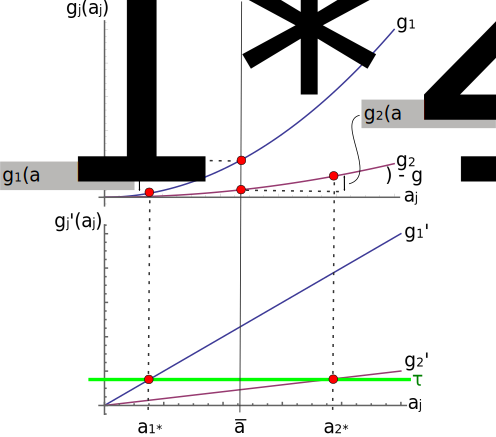
\includegraphics[width=0.8\textwidth]{2}
\caption{Two firms, both with quadratic abatement costs, face a Pigouvian tax $\tau$. They have resulting abatement responses $a_1^*$ and $a_2^*$. The average abatement $\abar$ is shown with the middle vertical line. The vertical difference for firm 1 between the abatement cost evaluated at $a_1^*$ and $\abar$ is greater than the vertical difference in firm 2's abatement cost evaluated at $a_2^*$ and $\abar$. Thus the welfare gain will be positive. However, because the second derivative of abatement costs are positive, the difference will be small for firms that have closer abatement cost curves (and thus a smaller spread of $\ajstar$'s).}
\label{fig1}
\end{figure}



% &= \sumj\left(\ajstar - \abar + \gamma_j\abar^2 - \gamma_j \ajstar^2\right)\\
% \intertext{Note that $\ajstar=\frac{1}{2\gamma_j}$ and $\abar=\frac{1}{J}\sumj\frac{1}{2\gamma_j}$, so}
% &= \sumj\left(\frac{1}{2\gamma_j} - \frac{1}{J}\sumk\frac{1}{2\gamma_k} 
%     + g_j\left(\frac{1}{J}\sumk\frac{1}{2\gamma_k}\right) 
%     - g_j\left(\frac{1}{2\gamma_j}\right)\right)\\




\FloatBarrier
\vspace{5em}
\newpage
%%%%%%%%%%%%%%%%%%%%%%%%%%%%%%%%%%%%%%%%%%%%%%%
%                Problem 3                    %
%%%%%%%%%%%%%%%%%%%%%%%%%%%%%%%%%%%%%%%%%%%%%%%
\vspace{5em}
\section*{Problem 3}

\problem{Two related dirty goods}{
    You wish to comment on the optimal tax for a good that creates a negative externality, but which is a relatively clean version of a product. That is, close substitutes for the good create an even larger externality. (I.e., you are thinking about taxing natural gas relative to coal; or hybrid cars relative to conventional vehicles; or energy-efficient appliances relative to less efficient ones.) Others debating this policy believe that the relatively clean product should be subsidized (not taxed) because the dirtier products are undertaxed relative to their marginal damages. You are not sure if the product should be subsidized, so you wish to describe the optimal tax on the relatively clean good, under the assumption that the dirtier substitute is undertaxed.\\
    
    \textbf{Write down a mathematical model that allows you to describe the optimal tax on the relatively clean good, assuming that the tax on the dirtier good is fixed and you cannot change it. Solve the model and describe how the results answer the broader question of how mispriced substitutes can affect optimal policy design for a dirty good.}
}


\textit{Note: I did not finish this problem. I realized that prices need to be endogenously determined and that I was working on an incomplete maximization problem. I then realized that Jacobsen et al. (2020) has the perfect model setup. I would need to add the budget constraint to the problem below, where the representative consumer has income and gets the tax revenue as additional funds.}


\def\qis{q_i^*} \def\qiss{q_i^{**}}

Adapting Holland, Hughes and Knittel (2009), let's define the following model:
\begin{itemize}
    \item Two fuel sources: $H$ and $L$ with high and low marginal damages, respectively.
    \item Assume perfectly competitive producers of both fuels.
    \item Associated productions costs $C_H(q), C_L(q)$ such that $C_H', C_H'', C_L', C_L''>0$ and $C_H(q)<C_L(q)\ \forall q>0$ (since dirtier fuels are often cheaper to produce per unit energy).
    \item Assume quantities $q_i$ of $C_H(q_H), C_L(q_L)$ are both measured in the same units of energy.
    \item Associated constant marginal damages $\phi_H, \phi_L$ such that $\phi_H>\phi_L\geq0$ so the environmental damage from fuel $i$ is $\phi_i q_i$.
    \item Let the social benefit from consumption of both types of energy be $U(q_H, q_L)$ such that $U$ is increasing, concave, and differentiable.
    \item There exists a fixed tax $t_H$ on the dirty fuel source such that $t_H < \phi_H$.
\end{itemize}
\begin{align*} 
\intertext{Then the social planner's problem becomes}
\max_{\{q_i\}} \SWF &= (\text{Benefit of consumption}) - (\text{Cost of production}) - (\text{Damages to the environment})\\
    &= U(q_H, q_L) - C_H(q_H) - C_L(q_L) - (\phi_H q_H + \phi_L q_L)
\intertext{and the FOCs for this are}
\part{U}{q_i}\Big|_{\qis} &= C_i'(\qis) + \phi_i \quad \text{for } i\in\{H,L\}
\intertext{Consider imposing two taxes $t_H, t_L$, where $t_H$ is fixed and $t_H < \phi_H$. Since we have perfect competition, the firms are price-takers and consider prices $p_i$ as exogenous. Then, assuming firms can choose to produce either or both fuels, a firm's profit maximization problem is}
\max_{\{q_i\}} \pi &= (\text{Revenue from selling the fuel}) - (\text{Cost of production}) - (\text{Tax payments})\\
    &= (p_H q_H + p_L q_L) - C_H(q_H) - C_L(q_L) - (t_H q_H + t_L q_L)
\intertext{and the firm's FOCs are:}
p_i &= C_i'(\qiss) + t_i
\intertext{Since consumers purchase until marginal benefit equals the price they pay, $p_i= \dpart{U}{q_i}\Big|_{\qiss}$ in equilibrium. Thus}
\part{U}{q_i}\Big|_{\qiss} &= C_i'(\qiss) + t_i
\intertext{Rearranging, we have}
\part{U}{q_i}\Big|_{\qiss} &- C_i'(\qiss)  = t_i
\intertext{We know $t_H < \phi_H$. Is $q_H^{**}$ larger or smaller than $q_H^*$? Since $U$ is increasing and concave (therefore decreasing slope) and $C_i$ is increasing in slope, the quantity on the left hand side increases as we decrease $\qiss$. i.e.,}
\frac{\partial}{\partial \qiss}&\left[\part{U}{q_i}\Big|_{\qiss} - C_i'(\qiss)\right]
    = \frac{\partial^2 U}{\partial q_i^2} - C_i'' <0
\intertext{Since $t_H < \phi_H$, then }
\part{U}{q_H}\Big|_{q_H^{**}} &- C_H'(q_H^{**}) < \part{U}{q_H}\Big|_{q_H^*} - C_H'(q_H^*)
\intertext{Since the function $\part{U}{q_i}\Big|_{q} &- C_i'(q)$ is unambiguously decreasing in $q$, it must be that $q_H^{**} > q_H^*$. Thus the quantity of the dirty good produced under the non-optimal tax will be greater than the first-best quantity. We knew this from the beginning -- the fuel that is undertaxed will be overproduced. But what is the optimal tax on the cleaner fuel?}
\intertext{We can pose the regulator's problem as setting the tax given the firms' best response function (their profit maximizing decision). The firm's best response for fuel $i$ is the quantity of $i$ produced given the price and tax:}
q_i(p_i, t_i) &= BR_i(p_i, t_i) = C_i'^{-1}(p_i - t_i)
\intertext{We treat $t_H$ as fixed, but the prices are determined endogenously between producers and consumers. So I write $p_i(t_L)$ as the equilibrium price of fuel $i$ resulting from tax $t_L$. Then using chain rule, we have}
\part{}{t_L}q_H(p_H, t_H) &= \part{q_H}{p_H}\part{p_H}{t_L} \\
\part{}{t_L}q_L(p_L, t_L) &= \part{q_L}{p_L}\part{p_L}{t_L} 
    + \part{q_L}{t_L}
\intertext{Since $q_i(p_i, t_i) = C_i'^{-1}(p_i - t_i)$, then}
\part{q_L}{t_L} &= -\part{q_L}{p_L} \quad \text{and} \quad
\part{}{t_L}q_L(p_L, t_L) = - \part{q_L}{t_L}\part{p_L}{t_L} 
    + \part{q_L}{t_L} = \part{q_L}{t_L}\left(1-\part{p_L}{t_L} \right)
\end{align*}


 

\end{document}

